% Figure 5.7: GNN Architecture for Career Path Prediction
% Compile with: pdflatex fig_5_7_gnn_architecture.tex

\documentclass[border=10pt]{standalone}
\usepackage{tikz}
\usetikzlibrary{shapes.geometric, arrows.meta, positioning}
\usepackage{xcolor}
\usepackage{amsmath}

% Professional academic color palette
\definecolor{inputgray}{RGB}{220, 220, 220}
\definecolor{embedblue}{RGB}{176, 196, 222}    % Light steel blue
\definecolor{gconvteal}{RGB}{119, 176, 166}    % Muted teal
\definecolor{denseorange}{RGB}{222, 184, 135}  % Burlywood
\definecolor{outputpurple}{RGB}{186, 175, 201} % Lavender gray
\definecolor{skillgreen}{RGB}{176, 208, 176}   % Sage green
\definecolor{careergray}{RGB}{180, 180, 180}   % Medium gray
\definecolor{textdark}{RGB}{33, 33, 33}

\begin{document}
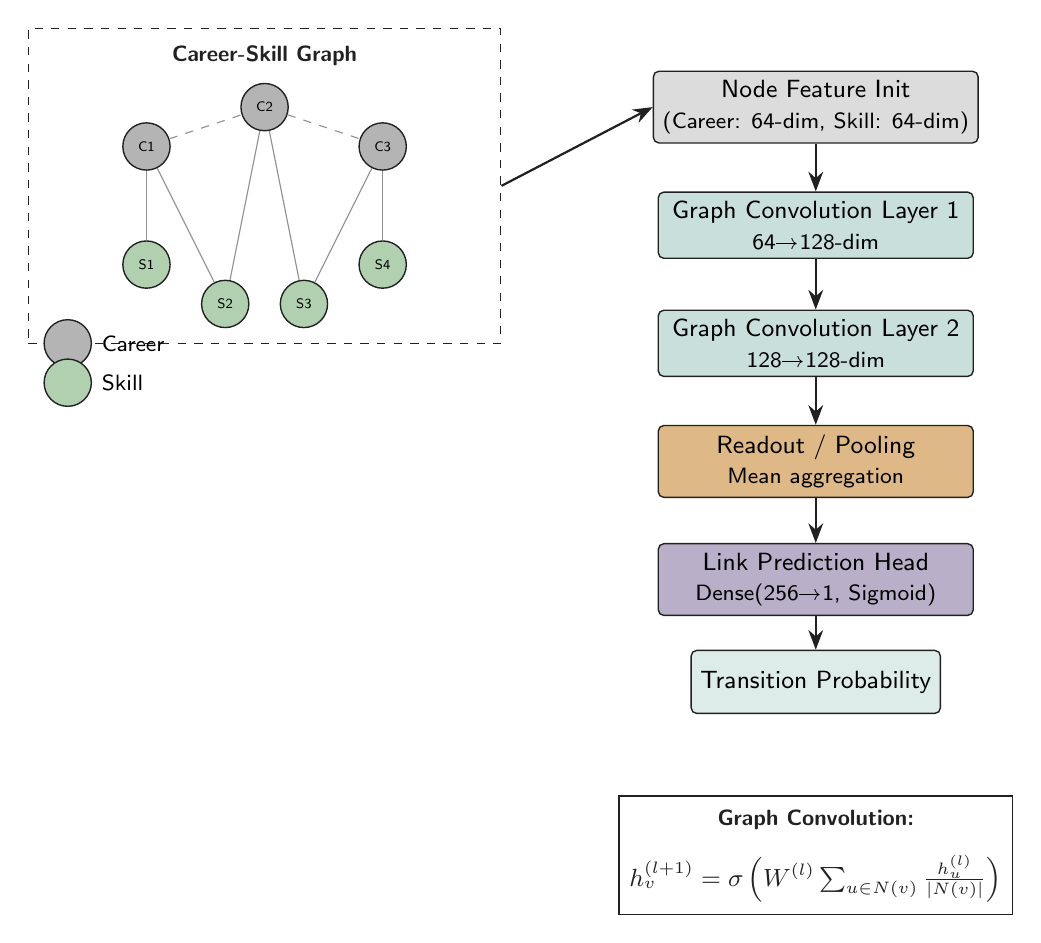
\begin{tikzpicture}[
    node distance=1cm,
    layer/.style={rectangle, draw=textdark, rounded corners=2pt, minimum width=2.5cm, minimum height=0.8cm, align=center, font=\small\sffamily, line width=0.5pt},
    gconv/.style={layer, fill=gconvteal!40},
    skillnode/.style={circle, draw=textdark, fill=skillgreen, minimum size=0.6cm, font=\tiny\sffamily, line width=0.5pt},
    careernode/.style={circle, draw=textdark, fill=careergray, minimum size=0.6cm, font=\tiny\sffamily, line width=0.5pt},
    arrow/.style={-{Stealth[length=2.5mm]}, thick, color=textdark},
]

% Graph visualization
\node[rectangle, draw=textdark, dashed, minimum width=6cm, minimum height=4cm, line width=0.5pt] (graph) at (-4, 5) {};
\node[font=\footnotesize\bfseries\sffamily, anchor=north, color=textdark] at (-4, 6.9) {Career-Skill Graph};

% Career nodes
\node[careernode] (c1) at (-5.5, 5.5) {C1};
\node[careernode] (c2) at (-4, 6) {C2};
\node[careernode] (c3) at (-2.5, 5.5) {C3};

% Skill nodes
\node[skillnode] (s1) at (-5.5, 4) {S1};
\node[skillnode] (s2) at (-4.5, 3.5) {S2};
\node[skillnode] (s3) at (-3.5, 3.5) {S3};
\node[skillnode] (s4) at (-2.5, 4) {S4};

% Edges
\draw[textdark!50] (c1) -- (s1);
\draw[textdark!50] (c1) -- (s2);
\draw[textdark!50] (c2) -- (s2);
\draw[textdark!50] (c2) -- (s3);
\draw[textdark!50] (c3) -- (s3);
\draw[textdark!50] (c3) -- (s4);
\draw[textdark!50, dashed] (c1) -- (c2);
\draw[textdark!50, dashed] (c2) -- (c3);

% Legend
\node[careernode, label=right:{\footnotesize\sffamily Career}] at (-6.5, 3) {};
\node[skillnode, label=right:{\footnotesize\sffamily Skill}] at (-6.5, 2.5) {};

% GNN Layers
\node[layer, fill=inputgray, minimum width=4cm] (init) at (3, 6) {Node Feature Init\\{\footnotesize\sffamily (Career: 64-dim, Skill: 64-dim)}};

\node[gconv, minimum width=4cm] (gc1) at (3, 4.5) {Graph Convolution Layer 1\\{\footnotesize\sffamily 64→128-dim}};

\node[gconv, minimum width=4cm] (gc2) at (3, 3) {Graph Convolution Layer 2\\{\footnotesize\sffamily 128→128-dim}};

\node[layer, fill=denseorange, minimum width=4cm] (readout) at (3, 1.5) {Readout / Pooling\\{\footnotesize\sffamily Mean aggregation}};

\node[layer, fill=outputpurple, minimum width=4cm] (pred) at (3, 0) {Link Prediction Head\\{\footnotesize\sffamily Dense(256→1, Sigmoid)}};

\node[layer, fill=gconvteal!25] (out) at (3, -1.3) {Transition Probability};

% Arrows
\draw[arrow] (graph.east) -- (init.west);
\draw[arrow] (init) -- (gc1);
\draw[arrow] (gc1) -- (gc2);
\draw[arrow] (gc2) -- (readout);
\draw[arrow] (readout) -- (pred);
\draw[arrow] (pred) -- (out);

% GCN equation
\node[rectangle, draw=textdark, minimum width=5cm, minimum height=1.5cm, line width=0.5pt] (eq) at (3, -3.5) {};
\node[font=\footnotesize\bfseries\sffamily, anchor=north, color=textdark] at (3, -2.8) {Graph Convolution:};
\node[font=\small, color=textdark] at (3, -3.8) {$h_v^{(l+1)} = \sigma\left(W^{(l)} \sum_{u \in N(v)} \frac{h_u^{(l)}}{|N(v)|}\right)$};

\end{tikzpicture}
\end{document}
